\documentclass{tufte-handout}
\usepackage[utf8]{inputenc}
\usepackage{tikz}
\usepackage{graphicx}
\usepackage{amsmath}

\usepackage{color}
\newcommand{\red}[1]{{\color{red} #1}}
\usepackage{booktabs}
\title{Red Scare!}
\begin{document}
\maketitle
\begin{abstract}
Oh no! All I wanted was to write a straightforward reachability exercise.
But some of the vertices have turned red, giving me cruel ideas for much harder questions! 
\end{abstract}
\section{Problems}
In every problem of this exercise, we consider a graph $G$ with vertex set $V(G)$ and edge set $E(G)$.
The graph can be directed or undirected.
Every graph in this exercise is simple (no multiple edges between any pair of vertices) and unweighted.
We fix the notation $n=|V(G)|$ and $m=|E(G)|$.

\begin{marginfigure}
 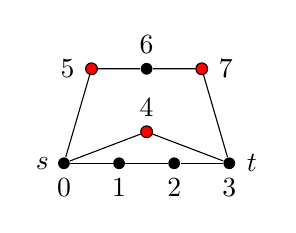
\begin{tikzpicture}[yscale=.4, xscale = .7]
 \begin{scope}[every node/.style={circle, fill, inner sep =1.5pt}]
   \node (0) [label=below:$0$, label = left:$s$] at (0,0) {};
   \node (1) [label=below:$1$] at (1,0) {};
   \node (2) [label=below:$2$] at (2,0) {};
   \node (3) [label=below:$3$, label = right:$t$] at (3,0) {};
   \node (4) [label=above:$4$, fill=red, draw, inner sep =1.5pt] at (1.5,1) {};
   \node (5) [label=left:$5$, fill=red, draw, inner sep =1.5pt] at (.5,3) {};
   \node (6) [label=above:$6$] at (1.5,3) {};
   \node (7) [label=right:$7$, fill=red, draw, inner sep =1.5pt] at (2.5,3) {};
   \draw (0) -- (1) -- (2) -- (3);
   \draw (0) -- (4) -- (3);
   \draw (0) -- (5) -- (6) -- (7) -- (3);
 \end{scope}
 \end{tikzpicture}
 \caption{Example graph $G_{\text{ex}}$ corresponding to the file {\tt G-ex}.}
\end{marginfigure}

Every graph comes with two specified vertices $s,t\in V(G)$ called the \emph{start} and \emph{end} vertices, and a subset $R\subseteq V(G)$ of \emph{red} vertices.
In particular, $R$ can inlude $s$ and $t$.
We fix the notation $r= |R|$.
In the example graph $G_{\text{ex}}$, we have $s=0$, $t=3$, and $R=\{4,5,7\}$.

An \emph{$s,t$-path} is a sequence of distinct vertices $v_1,\ldots, v_l$ such that $v_1=s$, $v_l=t$, and $v_iv_{i+1}\in E(G)$ for each $i\in\{1,\ldots,l-1\}$.
The \emph{length} of such a path is $l-1$, the number of edges.
Note that this definition requires the vertices on a path to be distinct, this is sometimes called a \emph{simple} path.

The problems we want solved for each graph are the following:
\begin{description}
  \item[None] Return the length of a shortest $s,t$-path internally avoiding $R$.
    To be precise, let $P$ be the set of $s,t$-paths using no vertices from $R$ except maybe $s$ and $t$ themselves. Let $l(p)$ denote the length of a path $p$.
    Return $\min\{\,l(p)\colon p\in P\,\}$.
    If no such path exists, return `-1'.
    Note that if the edge $st$ exists then the answer is 1, no matter the colour of $s$ or $t$.
    In $G_{\text{ex}}$, the answer is 3 (because of the path 0, 1, 2, 3.)
  \item[Some] Return `true' if there is a path from $s$ to $t$ that includes at least one vertex from $R$.
    Otherwise, return `false.'
    In $G_{\text{ex}}$, the answer is `yes' (in fact, two such paths exist: the path 0, 4, 3 and the path 0, 5, 6, 7, 3.)
  \item [Many] Return the maximum number of red vertices on any path from $s$ to $t$.
    To be precise, let $P$ be the set of $s,t$-paths and let $r(p)$ denote the number of red vertices  on a path $p$.
    Return $\max\{\,r(p)\colon p\in P\,\}$.
    If no path from $s$ to $t$ exists, return `-1'.
    In $G_{\text{ex}}$, the answer is `2' (because of the path 0, 5, 6, 7, 3.)
  \item [Few] Return the minimum number of red vertices on any path from $s$ to $t$.
    To be precise, let $P$ be the set of $s,t$-paths and let $r(p)$ denote the number of red vertices  on a path $p$.
    Return $\min\{\,r(p)\colon p\in P\,\}$.
    If no path from $s$ to $t$ exists, return `-1'.
    In $G_{\text{ex}}$, the answer is 0 (because of the path 0, 1, 2, 3.)
  \item [Alternate] Return `true' if there is a path from $s$ to $t$ that alternates between red and non-red vertices.
    To be precise, a path $v_1,\ldots, v_l$ is \emph{alternating} if for each $i\in\{1,\ldots,l-1\}$, exactly one endpoint of the edge $v_iv_{i+1}$ is red.
    Otherwise, return `false.'
    In $G_{\text{ex}}$, the answer is `yes' (because of the path 0, 5, 6, 7, 3.)
\end{description}

\subsection{Requirements}
\paragraph{Solved instances.}
For three of the problems (I’m not telling which), you need to be able to handle \emph{all} instances.
For the remaining two problems, you will not be able to solve all instances, but should be able to solve roughly half of them.
Your solutions must run in polynomial time. 
If you do have a polynomial-time implementation that takes more than 1 hour on some instance, just abort it and report this in your report.\sidenote{However, this should not happen. As a guideline, I have a non-optimised Python implementation that solves all the instances in a single run in half an hour on a low-powered 2012 laptop.}

For two of the problems (I’m not telling which), you will not be able to write an algorithm that works for all graphs, because the problems are hard in general.
For one of those problems, you should be able to argue for computational hardness with a simple reduction.
The other problem will probably mystify you.
A sophisticated hardness argument exists in the research literature (but not in the course text book)---you are welcome to try to find it and include a reference in your report.
But you are not required to find an explanation, and absolutely not required to come up with the reduction yourself. 

\paragraph{Universality.}
Your algorithms must run in polynomial time on a well-defined class of graphs.
“Well-defined class” means something like “all graphs,”\sidenote{“All graphs” means all simple, loop-less, unweighted graphs.} “directed graphs,” “undirected graphs,” “bipartite graphs,” “acyclic graphs,” “graphs of bounded treewidth,” “planar graphs,” “expanders” or even a combination of these.

In particular, you are allowed to do something like this: 
\begin{quotation}
  \vspace*{-3ex} \begin{tabbing}
  if \= (isBipartite($G$)) then\\
  \> $\cdots\qquad\qquad$\=\# run the Strumpf--Chosa algorithm \\
  else \\
  \> print(``?!'') \>\# problem is NP-hard for non-bipartite graphs, so give up
\end{tabbing}
\end{quotation}

On the other hand, you are not allowed to base your algorithm on specific knowledge of which graphs are in the {\tt data} directory,
For an extreme example, the following would not be allowed:
\begin{quotation}
  \vspace*{-3ex}
  \begin{tabbing}
  if \= (filename == "rusty-1-17")) then\\
  \> print("14") \=\# solved by hand\\
  else \\
  \> print(``?'') \>\# no idea what to do 
\end{tabbing}
\end{quotation}

\paragraph{Libraries.}
This exercise focusses on choosing \emph{between} algorithms, not implementing them.
Thus, you are \emph{not} required to write these algorithms from scratch.
For instance, if you need a minimum spanning tree, and you already have a working implementation of Prim’s algorithm, you are free to reuse that.
In particular, you are free to use a library implementation of these algorithms. 
You are also free to use implementations from books or from other people, provided that you are not violating any intellectual property rights.
(It goes without saying that you properly cite the source of these implementations in your report.)

You are highly encouraged to use your own implementation of standard graph algorithms that you may have made for some other exercise.
If you do this, then separate that implementation in your source code, maybe by leaving it in its own file. 
Attribute all the original authors in the source code.

\paragraph{Deliverables.}
Hand in 
\begin{enumerate}
  \item a report; follow the skeleton in {\tt doc/report.pdf}. 
  \item a text file {\tt results.txt} with all the results, as specified in the report.
  \item the programs you have written to answer the questions, including any scripts you need to run these programs on the instances, and a README file that explains how to recreate {\tt results.txt} by running your programs.
\end{enumerate}

\newpage
\section{Appendix: Gallery of Graphs}

This gallery consists of descriptions and drawings of many of the graphs in the {\tt data} directory.
Ideally, these descriptions are useful for finding mistakes in your code.
In particular, for many of these graphs it is obvious what the correct answers are.
Some of the graphs are \emph{random} graph---they have no structure and are pretty boring.
Others, such as the Word graphs, have a lot of structure.

\subsection{Individual graphs}
\begin{marginfigure}
 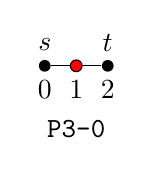
\begin{tikzpicture}[scale=.4]
   \node  at (1,-2) {\tt P3-0};
 \begin{scope}[every node/.style={circle, fill, inner sep =1.5pt}]
   \node (0) [label=below:$0$, label = above:$s$] at (0,0) {};
   \node (1) [label=below:$1$, fill=red, draw, inner sep =1.5pt] at (1,0) {};
   \node (2) [label=below:$2$, label = above:$t$] at (2,0) {};
   \draw (0) -- (1) -- (2);
 \end{scope}
 \end{tikzpicture}
\quad
 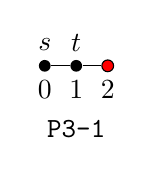
\begin{tikzpicture}[scale=.4]
   \node  at (1,-2) {\tt P3-1};
 \begin{scope}[every node/.style={circle, fill, inner sep =1.5pt}]
   \node (0) [label=below:$0$, label = above:$s$] at (0,0) {};
   \node (1) [label=below:$1$, label = above:$t$] at (1,0) {};
   \node (2) [label=below:$2$, fill=red, draw, inner sep =1.5pt] at (2,0) {};
   \draw (0) -- (1) -- (2);
 \end{scope}
 \end{tikzpicture}

 \bigskip
 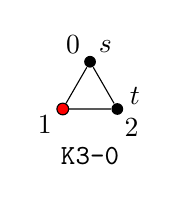
\begin{tikzpicture}[scale=.4]
   \node  at (0,-2) {\tt K3-0};
 \begin{scope}[every node/.style={circle, fill, inner sep =1.5pt}]
   \node (0) [label=135:$0$, label = 45:$s$] at (90:1cm) {};
   \node (1) [label=210:$1$, fill=red, draw, inner sep =1.5pt] at (210:1cm) {};
   \node (2) [label=285:$2$, label = 15:$t$] at (330:1cm) {};
   \draw (0) -- (1) -- (2) -- (0);
 \end{scope}
 \end{tikzpicture}
\quad
 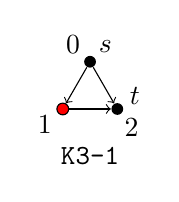
\begin{tikzpicture}[scale=.4]
   \node  at (0,-2) {\tt K3-1};
 \begin{scope}[every node/.style={circle, fill, inner sep =1.5pt}]
   \node (0) [label=135:$0$, label = 45:$s$] at (90:1cm) {};
   \node (1) [label=210:$1$, fill=red, draw, inner sep =1.5pt] at (210:1cm) {};
   \node (2) [label=285:$2$, label = 15:$t$] at (330:1cm) {};
   \draw [->] (0) -- (1);
   \draw [->] (1) -- (2);
   \draw [->] (0) -- (2);
 \end{scope}
 \end{tikzpicture}
\quad
 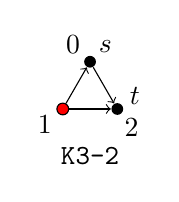
\begin{tikzpicture}[scale=.4]
   \node  at (0,-2) {\tt K3-2};
 \begin{scope}[every node/.style={circle, fill, inner sep =1.5pt}]
   \node (0) [label=135:$0$, label = 45:$s$] at (90:1cm) {};
   \node (1) [label=210:$1$, fill=red, draw, inner sep =1.5pt] at (210:1cm) {};
   \node (2) [label=285:$2$, label = 15:$t$] at (330:1cm) {};
   \draw [->] (1) -- (0);
   \draw [->] (1) -- (2);
   \draw [->] (0) -- (2);
 \end{scope}
 \end{tikzpicture}
 \caption{Paths and triangles with various choices of orientation and redness.}
 \end{marginfigure}

 The {\tt data} directory contains a small number of individual graphs, typicall of very small size.
 This includes $G_{\text{ex}}$, a number of small graphs of 3 vertices shown to the right, and an all-red dodecahedron.
 It is a good idea to use these graphs initially to ensure that your parser works, your graph data structure makes sense, etc.
These graphs also serve as an invitation to create more toy examples by hand while you test your code, so ensure that everything works on very small graphs.
Keep some good, clear drawings of `your' graphs around, they help immensely when finding mistakes.

\subsection{Word graphs}
In the word graphs, each vertex represents a five-letter word of English.
For $k\in\{1,2\}$, an edge joins $u$ and $v$ if the corresponding words are anagrams, or if they differ in exactly $k$ positions.
For instance ``begin'' and ``binge'' are neighbours, and so are ``turns'' and ``terns'' for $k=1$.

The word graphs  come in two flavours.
The \emph{rusty word} graphs are guaranteed to include ``begin,'' ``ender,'' and ``rusty.''
The vertex corresponding to ``rusty'' is coloured red, no other vertices are red.

The filenames are {\tt rusty-$k$-$n$}.
\begin{figure}
\[
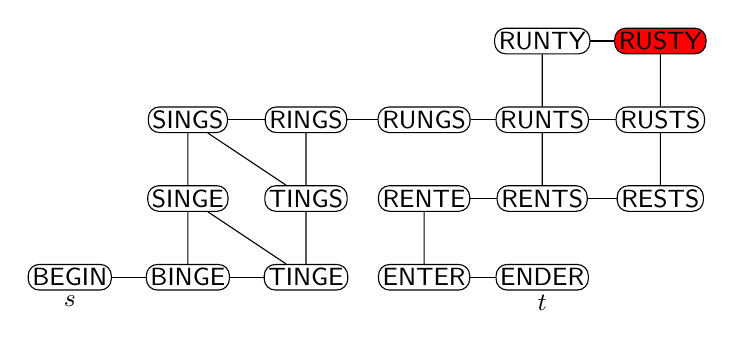
\begin{tikzpicture}[
    xscale = 1.5,
    every node/.style={ draw,rectangle,
      rounded corners, inner sep = 1.5pt, font =\sf\small }
    ]
  \node (rungs) at (3,2) {RUNGS}; 
  \node (sings) at (1,2) {SINGS}; 
  \node (begin) [label = below:$s$] at (0,0) {BEGIN};
  \node (rents) at (4,1) {RENTS};
  \node (ender) [label = below:$t$] at (4,0) {ENDER};
  \node (rests) at (5,1) {RESTS};
  \node (binge) at (1,0) {BINGE};
  \node (singe) at (1,1) {SINGE};
  \node (rings) at (2,2) {RINGS};
  \node (rusty) [fill = red] at (5,3) {RUSTY};
  \node (rente) at (3,1) {RENTE};
  \node (runts) at (4,2) {RUNTS};
  \node (enter) at (3,0) {ENTER};
  \node (rusts) at (5,2) {RUSTS};
  \node (tinge) at (2,0) {TINGE};
  \node (tings) at (2,1) {TINGS};
  \node (runty) at (4,3) {RUNTY};
\draw (rungs) -- (runts) ;
\draw (sings) -- (tings) ;
\draw (sings) -- (rings) ;
\draw (sings) -- (singe) ;
\draw (begin) -- (binge) ;
\draw (rents) -- (rests) ;
\draw (rents) -- (rente) ;
\draw (rents) -- (runts) ;
\draw (ender) -- (enter) ;
\draw (rests) -- (rusts) ;
\draw (binge) -- (tinge) ;
\draw (binge) -- (singe) ;
\draw (singe) -- (tinge) ;
\draw (rings) -- (tings) ;
\draw (rusty) -- (rusts) ;
\draw (rusty) -- (runty) ;
\draw (rente) -- (enter) ;
\draw (runts) -- (rusts) ;
\draw (runts) -- (runty) ;
\draw (tinge) -- (tings) ;
\draw (rungs) -- (rings) ;
  \end{tikzpicture}
\]
\caption{{\tt rusty-1-17}}
\end{figure}

The \emph{common word} use the same adjacency structure, and always include `start' and `ender.' 
A word is red if it is uncommon (like `ender'), just under half the words are uncommon.
The filenames for these graphs are {\tt common-$n$}.

\subsection{Grids}

\begin{marginfigure}
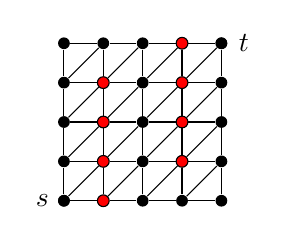
\begin{tikzpicture}[scale = .5, every node/.style={circle, fill, inner sep =1.5pt}]
  \foreach \x in {0,1,2,3,4} {
    \foreach \y in {0,1,2,3,4} {
      \node (\x_\y) at (\x,\y) {};
    }
  }
  \node [label = left:$s$] at (0,0) {};
  \node [label = right:$t$] at (4,4) {};
  \draw (1_4) -- (2_4);
  \draw (1_4) -- (0_4);
  \draw (1_4) -- (1_3);
  \draw (1_4) -- (0_3);
  \draw (1_3) -- (2_3);
  \draw (1_3) -- (2_4);
  \draw (1_3) -- (1_2);
  \draw (1_3) -- (0_2);
  \draw (1_3) -- (0_3);
  \draw (1_2) -- (2_2);
  \draw (1_2) -- (2_3);
  \draw (1_2) -- (1_1);
  \draw (1_2) -- (0_2);
  \draw (1_2) -- (0_1);
  \draw (1_1) -- (2_1);
  \draw (1_1) -- (2_2);
  \draw (1_1) -- (1_0);
  \draw (1_1) -- (0_0);
  \draw (1_1) -- (0_1);
  \draw (1_0) -- (2_0);
  \draw (1_0) -- (2_1);
  \draw (1_0) -- (0_0);
  \draw (0_4) -- (0_3);
  \draw (0_2) -- (0_3);
  \draw (0_2) -- (0_1);
  \draw (0_0) -- (0_1);
  \draw (3_1) -- (3_0);
  \draw (3_1) -- (3_2);
  \draw (3_1) -- (2_0);
  \draw (3_1) -- (2_1);
  \draw (3_1) -- (4_2);
  \draw (3_1) -- (4_1);
  \draw (3_0) -- (2_0);
  \draw (3_0) -- (4_0);
  \draw (3_0) -- (4_1);
  \draw (3_3) -- (3_2);
  \draw (3_3) -- (3_4);
  \draw (3_3) -- (2_2);
  \draw (3_3) -- (2_3);
  \draw (3_3) -- (4_3);
  \draw (3_3) -- (4_4);
  \draw (3_2) -- (2_1);
  \draw (3_2) -- (2_2);
  \draw (3_2) -- (4_2);
  \draw (3_2) -- (4_3);
  \draw (3_4) -- (2_3);
  \draw (3_4) -- (2_4);
  \draw (3_4) -- (4_4);
  \draw (2_0) -- (2_1);
  \draw (2_1) -- (2_2);
  \draw (2_2) -- (2_3);
  \draw (2_3) -- (2_4);
  \draw (4_2) -- (4_1);
  \draw (4_2) -- (4_3);
  \draw (4_3) -- (4_4);
  \draw (4_0) -- (4_1);
  \node [fill=red,draw,inner sep = 1.5pt] at (1,0) {};
  \node [fill=red,draw,inner sep = 1.5pt] at (1,1) {};
  \node [fill=red,draw,inner sep = 1.5pt] at (1,2) {};
  \node [fill=red,draw,inner sep = 1.5pt] at (1,3) {};
  \node [fill=red,draw,inner sep = 1.5pt] at (3,1) {};
  \node [fill=red,draw,inner sep = 1.5pt] at (3,2) {};
  \node [fill=red,draw,inner sep = 1.5pt] at (3,3) {};
  \node [fill=red,draw,inner sep = 1.5pt] at (3,4) {};
\end{tikzpicture}
\caption{The grid for $N=5$, represented by {\tt grid-5-0}.}
\end{marginfigure}

The Grid graphs consist of $N^2$ vertices that represent integer coordinates $(x,y)$ for $x,y\in\{0,\ldots,N-1\}$.
Each vertex $(x,y)$ is connected to $(x-1,y)$, $(x,y-1)$, and $(x-1,y-1)$, provided that these vertices exist.
The red vertices form a maze-like structure in the graph:
Every second row is red, except for the top- or bottommost vertex, alternatingly.
There is a unique $s,t$-path avoiding all red vertices, and a shortest alternating path following the diagonal.

Grid graphs of various sizes are represented by {\tt grid-$N$-0}.
Each of these graphs comes with two variants.
In {\tt grid-$N$-1}, some random red vertices have turned non-red (so there are `holes' in the hedges).
In {\tt grid-$N$-2}, some random non-red vertices have turned red (so some passages are blocked).


\subsection{Walls}

\begin{marginfigure}
 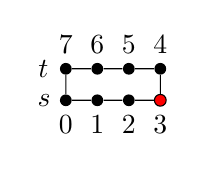
\begin{tikzpicture}[scale=.4]
 \begin{scope}[every node/.style={circle, fill, inner sep =1.5pt}]
   \node (0) [label=below:$0$, label=left:$s$] at (0,0) {};
   \node (1) [label=below:$1$] at (1,0) {};
   \node (2) [label=below:$2$] at (2,0) {};
   \node (3) [label=below:$3$,fill=red,draw,inner sep = 1.5pt] at (3,0) {};
   \node (4) [label=above:$4$] at (3,1) {};
   \node (5) [label=above:$5$] at (2,1) {};
   \node (6) [label=above:$6$] at (1,1) {};
   \node (7) [label=above:$7$, label=left:$t$] at (0,1) {};
   \draw (0) -- (1) -- (2) -- (3) -- (4) -- (5) -- (6) -- (7) -- (0);
 \end{scope}
 \end{tikzpicture}
 \caption{The single-brick wall, {\tt wall-p-1}.}
 \end{marginfigure}

Bricks are arranged like a wall of height $2$.
Here are three bricks with overlap $1$:
\begin{marginfigure}
 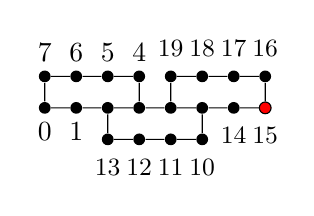
\begin{tikzpicture}[scale=.4]
 \begin{scope}[every node/.style={circle, fill, inner sep =1.5pt}]
   \node (0) [label=below:$0$] at (0,0) {};
   \node (1) [label=below:$1$] at (1,0) {};
   \node (2) [label=below:$$] at (2,0) {};
   \node (3) [label=below:$$] at (3,0) {};
   \node (4) [label=above:$4$] at (3,1) {};
   \node (5) [label=above:$5$] at (2,1) {};
   \node (6) [label=above:$6$] at (1,1) {};
   \node (7) [label=above:$7$] at (0,1) {};
   \node (8) [label=below:$$] at (4,0) {};
   \node (9) [label=below:$$] at (5,0) {};
   \node (10) [label=below:\small$10$]  at (5,-1) {};
   \node (11) [label=below:\small$11$]  at (4,-1) {};
   \node (12) [label=below:\small$12$]  at (3,-1) {};
   \node (13) [label=below:\small$13$]  at (2,-1) {};
   \node (14) [label=below:\small$14$]  at (6,0) {};
   \node (15) [label=below:\small$15$,fill=red,draw,inner sep = 1.5pt]  at (7,0) {};
   \node (16) [label=above:\small$16$]  at (7,1) {};
   \node (17) [label=above:\small$17$]  at (6,1) {};
   \node (18) [label=above:\small$18$]  at (5,1) {};
   \node (19) [label=above:\small$19$]  at (4,1) {};
   \draw (0) -- (1) -- (2) -- (3) -- (4) -- (5) -- (6) -- (7) -- (0);
   \draw (3)--(8)--(9)--(10)--(11)--(12)--(13)--(2);
   \draw (9)--(14)--(15)--(16)--(17)--(18)--(19)--(8);
 \end{scope}
 \end{tikzpicture}
 \caption{Three bricks with overlap 1, {\tt wall-p-3}.}
 \end{marginfigure}

 \begin{marginfigure}
 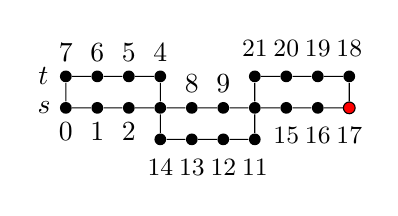
\begin{tikzpicture}[scale=.4]
 \begin{scope}[every node/.style={circle, fill, inner sep =1.5pt}]
   \node (0) [label=below:$0$, label=left:$s$] at (0,0) {};
   \node (1) [label=below:$1$] at (1,0) {};
   \node (2) [label=below:$2$] at (2,0) {};
   \node (3) [label=below:$$] at (3,0) {};
   \node (4) [label=above:$4$] at (3,1) {};
   \node (5) [label=above:$5$] at (2,1) {};
   \node (6) [label=above:$6$] at (1,1) {};
   \node (7) [label=above:$7$, label=left:$t$] at (0,1) {};
   \node (8) [label=above:$8$] at (4,0) {};
   \node (9) [label=above:$9$] at (5,0) {};
   \node (10) [label=below:\small$$]  at (6,0) {};
   \node (11) [label=below:\small$11$]  at (6,-1) {};
   \node (12) [label=below:\small$12$]  at (5,-1) {};
   \node (13) [label=below:\small$13$]  at (4,-1) {};
   \node (14) [label=below:\small$14$]  at (3,-1) {};
   \node (15) [label=below:\small$15$]  at (7,0) {};
   \node (16) [label=below:\small$16$]  at (8,0) {};
   \node (17) [label=below:\small$17$,fill=red,draw,inner sep = 1.5pt]  at (9,0) {};
   \node (18) [label=above:\small$18$]  at (9,1) {};
   \node (19) [label=above:\small$19$]  at (8,1) {};
   \node (20) [label=above:\small$20$]  at (7,1) {};
   \node (21) [label=above:\small$21$]  at (6,1) {};
   \draw (0) -- (1) -- (2) -- (3) -- (4) -- (5) -- (6) -- (7) -- (0);
   \draw (3)--(8)--(9)--(10)--(11)--(12)--(13)--(14)--(3);
   \draw (10)--(15)--(16)--(17)--(18)--(19)--(20)--(21)--(10);
 \end{scope}
 \end{tikzpicture}
 \caption{Three bricks with overlap 0, {\tt wall-z-3}.}
 \end{marginfigure}

 \begin{marginfigure}
 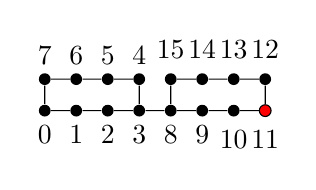
\begin{tikzpicture}[scale=.4]
 \begin{scope}[every node/.style={circle, fill, inner sep =1.5pt}]
   \node (0) [label=below:$0$] at (0,0) {};
   \node (1) [label=below:$1$] at (1,0) {};
   \node (2) [label=below:$2$] at (2,0) {};
   \node (3) [label=below:$3$] at (3,0) {};
   \node (4) [label=above:$4$] at (3,1) {};
   \node (5) [label=above:$5$] at (2,1) {};
   \node (6) [label=above:$6$] at (1,1) {};
   \node (7) [label=above:$7$] at (0,1) {};
   \node (8) [label=below:$8$] at (4,0) {};
   \node (9) [label=below:$9$] at (5,0) {};
   \node (10) [label=below:$10$]  at (6,0) {};
   \node (11) [label=below:$11$,fill=red,draw,inner sep = 1.5pt]  at (7,0) {};
   \node (12) [label=above:$12$]  at (7,1) {};
   \node (13) [label=above:$13$]  at (6,1) {};
   \node (14) [label=above:$14$]  at (5,1) {};
   \node (15) [label=above:$15$]  at (4,1) {};
   \draw (0) -- (1) -- (2) -- (3) -- (4) -- (5) -- (6) -- (7) -- (0);
   \draw (3)--(8)--(9)--(10)--(11)--(12)--(13)--(14)--(15)--(8);
 \end{scope}
 \end{tikzpicture}
 \caption{Two bricks with negative overlap, {\tt wall-n-2}.}
 \end{marginfigure}

The Wall graphs are a family consisting of $N$ overlapping 8-cycles called \emph{bricks}.
The bricks are laid in a wall of height 2, with various intervals of overlap.
Each wall has a single red vertex $w$, the rightmost vertex at the same level as vertex $0$.
These graphs are interesting instances for finding paths from $s$ to $t$ through the red vertex.
The should help you avoid some obvious pitfalls when developing an algorithm for the problem \emph{Some}.

The Walls with overlap 1, called {\tt brick-1-$N$}, allow an $s,t$-path through $w$.

The Walls with overlap 0, called {\tt brick-0-$N$}, allow a walk from $s$ to $t$ through $w$, but this walk will use $N-2$ vertices twice. 
In particular, such a walk it not a path, and your algorithm for Problem \emph{Some} should not be fooled by it.

The walls with negative overlap, called {\tt brick-n-$N$} also allow a walk from $s$ to $t$ through $w$, but this walk would use $N-2$ edges twice.
Again, such walk is not a path.

\section{Ski}
SkiFree\footnote{Read more at Wikipedia’s SkiFree page, the author’s site {\tt ski.ihoc.net}, or (amazingly) SkiFree Fan Fiction at {\tt www.fanfiction.net/game/SkiFree/}.} is an ancient computer game by Chris Pirih, part of the Microsoft Entertainment Pack in 1991, and going back to VT100 VAX/VMS terminals, ultimately inspired by Activision’s \emph{Skiing} for the Atari 2600 console.

Time to show you can handle yourself off-pist. Get from the start to the goal, avoiding the trees, dogs rocks etc.
Beware of the dreaded Yeti who is told to lurk at the red nodes of the mountain and will certainly chase you down and eat you if you pass him.

In each level, the player moves down, and either one step left or right.
(Some moves are blocked by obstacles.)

\begin{figure*}[h]
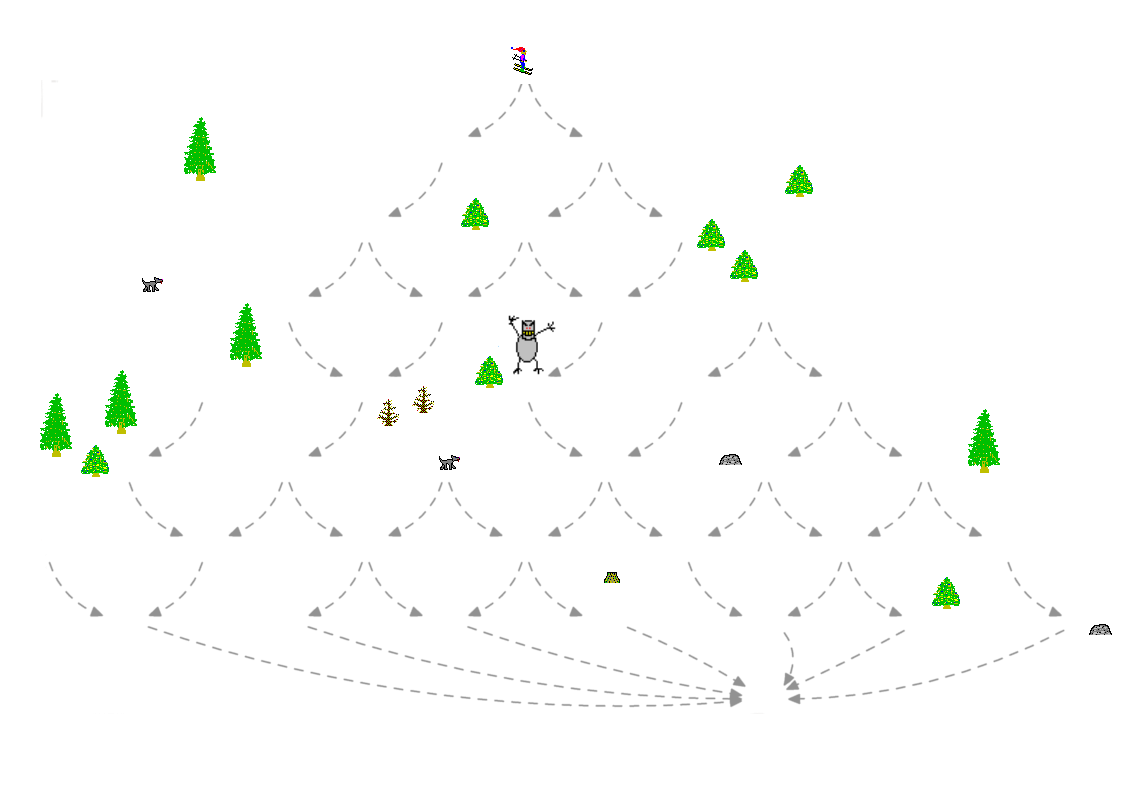
\includegraphics[width=7cm]{ski.png}  
\quad
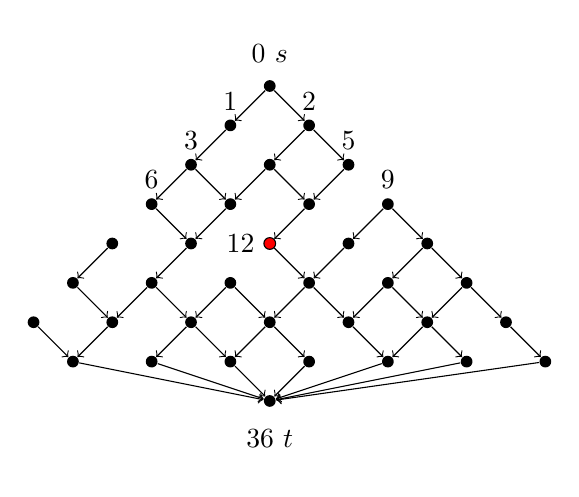
\begin{tikzpicture}[scale = .5, every node/.style={circle, fill, inner sep =1.5pt}]
  \node  (0) [label = above:$0\,\,s$] at (0,0) {};
  \node  (1) [label = above:$1$] at (-1,-1) {};
  \node  (2) [label = above:$2$] at (1,-1) {};
  \node  (3) [label = above:$3$] at (-2,-2) {};
  \node  (4) at (0,-2) {};
  \node  (5) [label = above:$5$] at (2,-2) {};
  \node  (6) [label = above:$6$] at (-3,-3) {};
  \node  (7) at (-1,-3) {};
  \node  (8) at (1,-3) {};
  \node  (9) [label = above:$9$] at (3,-3) {};
  \node (10) at (-4,-4) {};
  \node (11) at (-2,-4) {};
  \node (12) [label = left:$12$, fill = red, draw] at (0,-4) {};
  \node (13) at (2,-4) {};
  \node (14) at (4,-4) {};
  \node (15) at (-5,-5) {};
  \node (16) at (-3,-5) {};
  \node (17) at (-1,-5) {};
  \node (18) at (1,-5) {};
  \node (19) at (3,-5) {};
  \node (20) at (5,-5) {};
  \node (21) at (-6,-6) {};
  \node (22) at (-4,-6) {};
  \node (23) at (-2,-6) {};
  \node (24) at (0,-6) {};
  \node (25) at (2,-6) {};
  \node (26) at (4,-6) {};
  \node (27) at (6,-6) {};
  \node (29) at (-5,-7) {};
  \node (30) at (-3,-7) {};
  \node (31) at (-1,-7) {};
  \node (32) at (1,-7) {};
  \node (33) at (3,-7) {};
  \node (34) at (5,-7) {};
  \node (35) at (7,-7) {};
  \node (36) [label= below:$36\,\,t$] at (0,-8) {};
  \draw [->] (0) -- (1);
  \draw [->] (0) -- (2);
  \draw [->] (1) -- (3);
  \draw [->] (2) -- (4);
  \draw [->] (2) -- (5);
  \draw [->] (3) -- (6);
  \draw [->] (3) -- (7);
  \draw [->] (4) -- (7);
  \draw [->] (4) -- (8);
  \draw [->] (5) -- (8);
  \draw [->] (6) -- (11);
  \draw [->] (7) -- (11);
  \draw [->] (8) -- (12);
  \draw [->] (9) -- (13);
  \draw [->] (9) -- (14);
  \draw [->] (10) -- (15);
  \draw [->] (11) -- (16);
  \draw [->] (12) -- (18);
  \draw [->] (13) -- (18);
  \draw [->] (14) -- (19);
  \draw [->] (14) -- (20);
  \draw [->] (15) -- (22);
  \draw [->] (16) -- (22);
  \draw [->] (16) -- (23);
  \draw [->] (17) -- (23);
  \draw [->] (17) -- (24);
  \draw [->] (18) -- (24);
  \draw [->] (18) -- (25);
  \draw [->] (19) -- (25);
  \draw [->] (19) -- (26);
  \draw [->] (20) -- (26);
  \draw [->] (20) -- (27);
  \draw [->] (21) -- (29);
  \draw [->] (22) -- (29);
  \draw [->] (23) -- (30);
  \draw [->] (23) -- (31);
  \draw [->] (24) -- (31);
  \draw [->] (24) -- (32);
  \draw [->] (25) -- (33);
  \draw [->] (26) -- (33);
  \draw [->] (26) -- (34);
  \draw [->] (27) -- (35);
  \draw [->] (29) -- (36);
  \draw [->] (30) -- (36);
  \draw [->] (31) -- (36);
  \draw [->] (32) -- (36);
  \draw [->] (33) -- (36);
  \draw [->] (34) -- (36);
  \draw [->] (35) -- (36);
\end{tikzpicture}
\caption{A Ski level and the corresponding graph.
  This graph is described in {\tt ski-illustration}.
Yeti is lurking at node 12.
Graphics from {\tt ski.ihoc.net}.}
\end{figure*}

\subsection{Increasing numbers}
Each \emph{Increase} graph is generated from a sequence $a_1,\ldots, a_n$ of unique integers with $0\leq\alpha_i\leq 2n$.
(The random process is this: Pick a subset of size $n$ from $\{0,\ldots, 2n\}$ and arrange the elements in random order.)
We set $s=\alpha_1$ and $t=\alpha_n$.
Odd numbers are red.
There is an edge from  $\alpha_i$ to $\alpha_j$ if $i<j$ and $\alpha_i<\alpha_j$.

\begin{figure}
 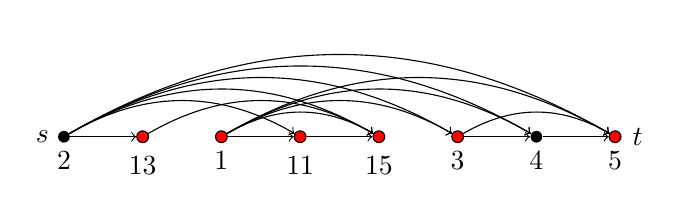
\begin{tikzpicture}[]
 \begin{scope}[every node/.style={circle, fill, inner sep =1.5pt}]
   \node (2)  [label=below:$2$, label = left:$s$] at (0,0) {};
   \node (13) [label=below:$13$, fill=red, draw] at (1,0) {};
   \node (1)  [label=below:$1$,  fill=red, draw] at (2,0) {};
   \node (11) [label=below:$11$, fill=red, draw] at (3,0) {};
   \node (15) [label=below:$15$, fill=red, draw] at (4,0) {};
   \node (3)  [label=below:$3$,  fill=red, draw] at (5,0) {};
   \node (4)  [label=below:$4$] at (6,0) {};
   \node (5)  [label=below:$5$, label = right:$t$, fill=red, draw] at (7,0) {};
   \draw [->] (2) edge[] (13);
   \draw [->] (2) edge [bend left] (11);
   \draw [->] (2) edge [bend left] (15);
   \draw [->] (2) edge [bend left] (3);
   \draw [->] (2) edge [bend left] (4);
   \draw [->] (2) edge [bend left] (5);
   \draw [->] (13) edge [bend left] (15);
   \draw [->] (1) edge [] (11);
   \draw [->] (1) edge [bend left] (15);
   \draw [->] (1) edge [bend left] (3);
   \draw [->] (1) edge [bend left] (4);
   \draw [->] (1) edge [bend left] (5);
   \draw [->] (11) edge []  (15);
   \draw [->] (3) edge [] (4);
   \draw [->] (3) edge [bend left] (5);
   \draw [->] (4) edge [] (5);
 \end{scope}
 \end{tikzpicture}
 \caption{\tt increase-n8-1.0}
  \end{figure}


\begin{figure}
 \begin{tikzpicture}[]
 \begin{scope}[every node/.style={circle, fill, inner sep =1.5pt}]
   \node (11)  [label=below:$11$, label = left:$s$] at (0,0) {};
   \node (15) [label=below:$15$, fill=red, draw] at (1,0) {};
   \node (1)  [label=below:$1$,  fill=red, draw] at (2,0) {};
   \node (8) [label=below:$8$] at (3,0) {};
   \node (13) [label=below:$13$, fill=red, draw] at (4,0) {};
   \node (4)  [label=below:$4$] at (5,0) {};
   \node (6)  [label=below:$6$] at (6,0) {};
   \node (12)  [label=below:$12$, label = right:$t$] at (7,0) {};
   \draw [->] (11) edge[] (15);
   \draw [->] (11) edge [bend left] (13);
   \draw [->] (11) edge [bend left] (12);
   \draw [->] (1) edge [] (8);
   \draw [->] (1) edge [bend left] (13);
   \draw [->] (1) edge [bend left] (3);
   \draw [->] (1) edge [bend left] (4);
   \draw [->] (1) edge [bend left] (6);
   \draw [->] (1) edge [bend left] (12);
   \draw [->] (8) edge [] (13);
   \draw [->] (8) edge [bend left] (12);
   \draw [->] (4) edge [] (6);
   \draw [->] (4) edge [bend left] (12);
 \end{scope}
 \end{tikzpicture}
 \caption{\tt increase-n8-2.0}
  \end{figure}

\end{document}
